% Slides: the API of the MACE consensus loop and of the 4D reconstruction
% model in mbirtorch, on branch mace_4d_dev.  The look follows the
% mbirtorch update deck of September 2026 (metropolis theme, one accent).
% Build: latexmk -pdf main.tex, or compile on Overleaf with pdfLaTeX.
\documentclass[aspectratio=169,10pt]{beamer}
\usepackage[T1]{fontenc}
\usepackage[utf8]{inputenc}
\usetheme[progressbar=frametitle,numbering=fraction]{metropolis}
\usepackage[sfdefault,lining]{FiraSans}
\usepackage{FiraMono}
\usepackage{graphicx}
\usepackage{array}
\usepackage{colortbl}
\usepackage{calc}
\usepackage{listings}
\usepackage[most]{tcolorbox}
\usepackage{tikz}
\usetikzlibrary{positioning,arrows.meta,calc,fit}

\definecolor{planAccent}{HTML}{3D6B99}   % accent, note bars, MACE boxes
\definecolor{axialBrick}{HTML}{A23B3B}   % the feedback arrow
\definecolor{safeGreen}{HTML}{2E7D32}    % data fit boxes, MACE4D chip
\definecolor{branchAmber}{HTML}{B26B1F}  % status chip
\definecolor{inkGray}{HTML}{5A5A5A}
\definecolor{barGray}{HTML}{262626}

% Code colors: the Pygments "default" style that Sphinx uses in light mode.
\definecolor{codeBg}{HTML}{F8F8F8}
\definecolor{pyKeyword}{HTML}{008000}
\definecolor{pyString}{HTML}{BA2121}
\definecolor{pyComment}{HTML}{3D7B7B}

\setbeamercolor{frametitle}{bg=barGray, fg=white}

% A chip in the frame title bar.
\newcommand{\tagchip}[2]{{\setlength{\fboxsep}{2.5pt}\setlength{\fboxrule}{0.6pt}%
  \fcolorbox{white}{#1}{\textcolor{white}{\footnotesize\bfseries\strut #2}}}}
\newcommand{\onbranch}{\tagchip{branchAmber}{BRANCH}}
\newcommand{\macechip}{\tagchip{planAccent}{MACE}}
\newcommand{\fourdchip}{\tagchip{safeGreen}{MACE4D}}

\newcommand{\speclabel}[1]{\textcolor{inkGray}{\scriptsize\MakeUppercase{#1}}}

% A note with the accent bar.
\newsavebox{\notebox}
\newcommand{\footnoteline}[1]{%
  \savebox{\notebox}{\begin{minipage}[b]{0.94\linewidth}\raggedright
    {\footnotesize\textcolor{inkGray}{#1}}\end{minipage}}%
  {\color{planAccent}\rule[-\dp\notebox]{2pt}{\dimexpr\ht\notebox+\dp\notebox\relax}}%
  \hspace{6pt}\usebox{\notebox}}

\newcommand{\source}[1]{\par\vfill{\scriptsize\textcolor{inkGray}{Source: #1}\par}}
\newcommand{\figcaption}[1]{{\scriptsize\textcolor{inkGray}{#1}\par}}
\newcommand{\head}[1]{\textbf{#1}}
\newcommand{\rowrule}{\arrayrulecolor{inkGray!35}\hline\noalign{\vskip 2pt}}

% A signature in the form of the Sphinx documentation: a gray bar with the
% qualified name and the argument list, then a "Parameters" list.
\newtcolorbox{sigbox}{enhanced jigsaw, colback=black!5, colframe=black!5,
  boxrule=0pt, arc=1pt, left=6pt, right=4pt, top=3pt, bottom=3pt, boxsep=0pt,
  borderline west={2.5pt}{0pt}{planAccent}, before skip=2pt, after skip=2pt}
\newcommand{\sig}[3]{\begin{sigbox}\raggedright\scriptsize\hangindent=14pt\hangafter=1
  \textit{#1} \texttt{\textbf{#2}(#3)}\end{sigbox}}
\newenvironment{params}{\par{\scriptsize\textbf{Parameters:}}\par\vspace{-6pt}%
  \begin{itemize}\scriptsize\setlength{\itemsep}{0pt}\setlength{\topsep}{0pt}}{\end{itemize}\vspace{-2pt}}
\newcommand{\param}[3]{\item \texttt{#1} (\textit{#2}) -- #3}
\newcommand{\returns}[1]{\par{\scriptsize\textbf{Returns:} #1\par}}
\newcommand{\sigtext}[1]{{\scriptsize #1\par}}

% Python examples.
\lstset{
  language=Python,
  basicstyle=\ttfamily\scriptsize,
  backgroundcolor=\color{codeBg},
  keywordstyle=\color{pyKeyword}\bfseries,
  commentstyle=\color{pyComment}\itshape,
  stringstyle=\color{pyString},
  emph={print,range,len},
  emphstyle=\color{pyKeyword},
  showstringspaces=false,
  columns=flexible,
  keepspaces=true,
  frame=none,
  xleftmargin=4pt,
  framexleftmargin=4pt,
  aboveskip=2pt,
  belowskip=2pt,
}

\title{The MACE and MACE4D API in mbirtorch}
\subtitle{The consensus loop, its agents, and 4D reconstruction}
\author{Ziyun Li}
\date{September 2026}

\begin{document}

\maketitle

% ================================================================ purpose
\begin{frame}{What these slides cover}
  \medskip
  {\large Two classes on the \texttt{mace\_4d\_dev} branch of mbirtorch:
  the \texttt{MACE} loop and the \texttt{MACE4DModel} built on it.}\par\vspace{8pt}
  {\small
  \head{Part 1, the MACE loop.}  Multi-agent consensus equilibrium (MACE)
  reconstructs one image from several agents.  An agent is any function
  that takes an image and returns the image it prefers.  The loop finds an
  image that every agent agrees on.\par\vspace{6pt}
  \head{Part 2, the 4D model.}  \texttt{MACE4DModel} reconstructs one
  volume per time frame from one continuous scan of a moving object.  It
  is a MACE loop with four agents that the model builds for the
  user.\par\vspace{6pt}
  \head{Reading the slides.}  Each slide states the idea first and the
  details after.  Constructors and methods with an argument list are shown
  in the form of the Sphinx documentation.  Every fact is taken from the
  code and docstrings named at the foot of the slide.  All of this code is
  complete on the branch and not yet released.}
\end{frame}

% ================================================================ the two classes
\begin{frame}{The two classes in one picture \hfill \onbranch}
  \centering
  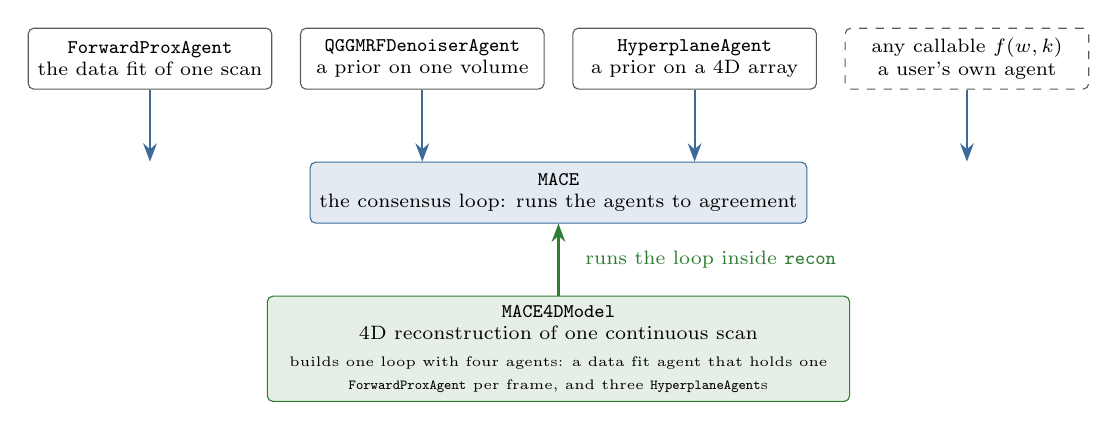
\begin{tikzpicture}[>=Stealth, node distance=8pt and 10pt,
      box/.style={draw, rounded corners=2pt, minimum height=22pt, font=\scriptsize, align=center},
      loop/.style={box, fill=planAccent!14, draw=planAccent, minimum width=150pt},
      agent/.style={box, fill=white, draw=inkGray, minimum width=88pt},
      user/.style={box, fill=safeGreen!12, draw=safeGreen, minimum width=150pt, inner xsep=8pt}]
    \node[agent] (a1) {\texttt{ForwardProxAgent}\\ the data fit of one scan};
    \node[agent, right=of a1] (a2) {\texttt{QGGMRFDenoiserAgent}\\ a prior on one volume};
    \node[agent, right=of a2] (a3) {\texttt{HyperplaneAgent}\\ a prior on a 4D array};
    \node[agent, right=of a3, dashed] (a4) {any callable $f(w, k)$\\ a user's own agent};
    \node[loop, below=26pt of $(a2.south)!0.5!(a3.south)$] (mace) {\texttt{MACE}\\ the consensus loop: runs the agents to agreement};
    \node[user, below=26pt of mace] (m4d) {\texttt{MACE4DModel}\\ 4D reconstruction of one continuous scan\\[2pt]
      \tiny builds one loop with four agents: a data fit agent that holds one\\ \tiny \texttt{ForwardProxAgent} per frame, and three \texttt{HyperplaneAgent}s};
    \foreach \a in {a1,a2,a3,a4} {
      \draw[->, planAccent, thick] (\a.south) -- (mace.north -| \a.south);
    }
    \draw[->, safeGreen, thick] (m4d.north) -- (mace.south)
      node[midway, right=6pt, font=\scriptsize, safeGreen] {runs the loop inside \texttt{recon}};
  \end{tikzpicture}\\[8pt]
  \figcaption{An agent is passed to the loop as a list entry.  A user who
  writes a plain function can pass it to \texttt{MACE} directly.  The 4D
  model constructs its own agents and runs the loop inside its
  \texttt{recon} method.}
  \source{\texttt{mbirtorch/mace.py}; \texttt{mbirtorch/mace4d.py}}
\end{frame}

% ================================================================ PART 1
\section{Part 1: the MACE loop}

% ---------------------------------------------------------------- the idea
\begin{frame}{The idea: several agents agree on one image \hfill \macechip}
  \begin{columns}[T]
    \begin{column}{0.50\textwidth}
      {\footnotesize
      \head{An agent} is a function from an image to an image of the same
      shape.  It returns the image it prefers.  One example is the proximal
      map of a data fit term, which pulls the image toward the measured
      data.  Another is a denoiser, which pulls the image toward a smooth
      one.\par\vspace{5pt}
      \head{The loop} keeps one input $W_k$ per agent.  In each step it
      evaluates every agent, forms a weighted average of the outputs, and
      moves each input toward that average.  At a fixed point every agent
      returns the same image, and that image is the result.\par\vspace{5pt}
      \head{Two numbers control it.}  The weights $\mu_k$ say how much each
      agent counts and sum to one.  The step $\rho$ says how far each input
      moves per step.  With two agents, equal weights, and $\rho = 1/2$,
      the loop is the same iteration ADMM uses.\par}
    \end{column}
    \begin{column}{0.48\textwidth}
      \centering
      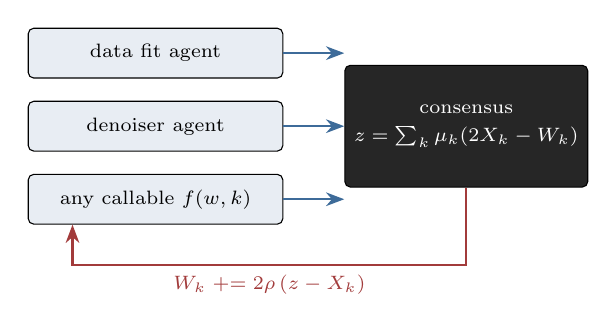
\begin{tikzpicture}[>=Stealth, node distance=8pt and 22pt,
          agent/.style={draw, rounded corners=2pt, fill=planAccent!12, minimum width=92pt, minimum height=18pt, font=\scriptsize},
          cons/.style={draw, rounded corners=2pt, fill=barGray, text=white, minimum width=70pt, minimum height=44pt, font=\scriptsize, align=center}]
        \node[agent] (a1) {data fit agent};
        \node[agent, below=of a1] (a2) {denoiser agent};
        \node[agent, below=of a2] (a3) {any callable $f(w, k)$};
        \node[cons, right=of a2] (c) {consensus\\[2pt] $z=\sum_k \mu_k (2X_k - W_k)$};
        \foreach \a in {a1,a2,a3} {
          \draw[->, planAccent, thick] (\a.east) -- (c.west |- \a.east);
        }
        \draw[->, axialBrick, thick] (c.south) -- ++(0,-28pt) -| ($(a3.south)+(-30pt,0)$)
          node[pos=0.25, below, font=\scriptsize, axialBrick] {$W_k \mathrel{+}= 2\rho\,(z - X_k)$};
      \end{tikzpicture}\\[6pt]
      \figcaption{Each agent maps its input $W_k$ to an output $X_k$.  The
      loop forms the consensus point $z$ from the outputs and moves every
      input toward it.  The reported result is the weighted average
      $\bar{x} = \sum_k \mu_k X_k$.}
    \end{column}
  \end{columns}
  \source{module docstring of \texttt{mbirtorch/mace.py}}
\end{frame}

% ---------------------------------------------------------------- the class, part 1
\begin{frame}{The \texttt{MACE} class: constructing and running it \hfill \macechip}
  \vspace{2pt}
  \sig{class}{mbirtorch.mace.MACE}{agents, x0, mu=None, rho=0.5, devices=None}
  \begin{params}
    \param{agents}{list}{the agents.  Each is a callable \texttt{agent(w, iteration)} that returns a tensor of the shape of \texttt{w} on the device of \texttt{w}.  Two later slides give the optional additions.}
    \param{x0}{numpy or tensor}{the initial image.  Every agent input starts here, and the state lives on its device.}
    \param{mu}{list of float, optional}{the agent weights, which sum to one.  Defaults to equal weights.}
    \param{rho}{float, optional}{the step of the consensus iteration, in (0, 1).  Defaults to 0.5.}
    \param{devices}{optional}{None runs every task in order on the calling thread.  Otherwise a device pool, in any form of the next slides, with one worker thread per entry.}
  \end{params}
  \vspace{3pt}
  \sig{method}{run}{max\_iterations=30, stop\_threshold\_change\_pct=0.0, callback=None}
  \sigtext{Steps until the percent change of the average falls below the
  threshold or \texttt{max\_iterations} steps have run in total.
  \texttt{callback(iteration, x\_bar)} is called after each step.}
  \returns{\texttt{(x\_bar, info)}, the consensus average and the traces.}
  \vspace{3pt}
  \sigtext{\texttt{step()} runs one iteration and returns the percent
  change.  \texttt{close()} stops the worker threads, as does leaving a
  \texttt{with MACE(...) as loop:} block.  \texttt{mu} and \texttt{rho} are
  plain attributes, so a caller may change them between steps.}
  \source{class docstring of \texttt{MACE} in \texttt{mbirtorch/mace.py}}
\end{frame}

% ---------------------------------------------------------------- the class, part 2
\begin{frame}{The \texttt{MACE} class: its state, traces, and memory \hfill \macechip}
  \vspace{0pt}
  {\small The state can be read, saved, and restored, so a long run can be
  resumed in a later process.}\par\vspace{4pt}
  {\scriptsize
  \begin{tabular}{@{}>{\raggedright\arraybackslash}p{0.30\linewidth}@{\hspace{6pt}}>{\raggedright\arraybackslash}p{0.66\linewidth}@{}}
    \speclabel{attributes} & \\[2pt]
    \texttt{W} & the agent inputs, one tensor per agent \\[2pt]
    \texttt{x\_bar} & the consensus average after the last step.  It is the loop's own buffer, and the next step overwrites it, so a caller who keeps it clones it. \\[2pt]
    \texttt{iteration} & the steps completed \\[2pt]
    \texttt{info} & per step traces, one list entry per step: \texttt{change\_pct}, the percent change of the average; \texttt{spread}, one value per agent, the distance of its output from the previous average; \texttt{time}, the wall time of the step; \texttt{tasks}, the start and end time of every task and the worker it ran on \\[6pt]
    \speclabel{checkpoints} & \\[2pt]
    \texttt{state\_dict()} & the inputs, the average, the count, the traces, and each agent's own state where the agent provides one \\[2pt]
    \texttt{load\_state\_dict(state)} & restores that into a loop whose agents and array shape match.  The loop keeps its own \texttt{mu} and \texttt{rho}, and warns when the saved ones differ. \\
  \end{tabular}}
  \vfill
  \footnoteline{Memory: each agent's output is added into the average as it
  arrives, so the loop holds three full size arrays beyond the agent
  inputs, whatever the number of agents.}
  \source{class docstring of \texttt{MACE} in \texttt{mbirtorch/mace.py}}
\end{frame}

% ---------------------------------------------------------------- vocabulary
\begin{frame}{Devices, workers, and tasks: what they are and who owns them \hfill \macechip}
  \begin{columns}[T]
    \begin{column}{0.50\textwidth}
      {\footnotesize
      \head{A device} is one GPU or the CPU, a \texttt{torch.device}.
      \head{The pool} is the list of devices the loop may use.  The caller
      chooses it once, through \texttt{devices=} or, for the 4D model,
      \texttt{set\_device\_pool}.\par\vspace{5pt}
      \head{A worker} is one thread bound to one device of the pool.  The
      loop creates the workers at its first step, one per pool entry, and
      stops them in \texttt{close()}.  With no pool there are no workers,
      and tasks run one after another on the calling thread.\par\vspace{5pt}
      \head{A task} is one piece of an agent's work.  It names a region
      of the array, a function that computes the agent's output over that
      region on a given device, and the device it must run on, or None
      for any.  A large agent divides its work into tasks so that the
      pieces run on different GPUs at the same time and no GPU holds the
      whole array.  A small agent provides no tasks, and the loop treats
      its one call as a single task over the whole array.\par}
    \end{column}
    \begin{column}{0.48\textwidth}
      {\scriptsize
      \begin{tabular}{@{}>{\raggedright\arraybackslash}p{0.17\linewidth}@{\hspace{5pt}}>{\raggedright\arraybackslash}p{0.30\linewidth}@{\hspace{5pt}}>{\raggedright\arraybackslash}p{0.20\linewidth}@{\hspace{5pt}}>{\raggedright\arraybackslash}p{0.20\linewidth}@{}}
        \speclabel{object} & \speclabel{made by} & \speclabel{owned by} & \speclabel{lives for} \\[3pt]
        agent & the caller & the caller & the caller decides \\[3pt]
        \rowrule
        pool & the caller & the loop & the loop \\[3pt]
        \rowrule
        worker & the loop, at its first step & the loop & until \texttt{close()} \\[3pt]
        \rowrule
        task & the agent, at each step & the step & one step \\[3pt]
        \rowrule
        the arrays & the loop, from \texttt{x0} & the loop & the loop \\
      \end{tabular}}\par\vspace{8pt}
      {\footnotesize
      \head{The loop's arrays} are one input $W_k$ per agent and the
      running average.  When a task returns, the loop adds its output into
      the part of those arrays that the task's region covers.  A lock
      makes the additions one at a time, so two tasks that finish together
      cannot corrupt the sum.  An error in any task is raised again on
      the calling thread.\par}
    \end{column}
  \end{columns}
  \source{\texttt{Task}, \texttt{MACE.step}, and the worker class in \texttt{mbirtorch/mace.py}}
\end{frame}

% ---------------------------------------------------------------- devices
\begin{frame}{How one step spreads its tasks over the pool \hfill \macechip}
  \begin{columns}[T]
    \begin{column}{0.50\textwidth}
      {\footnotesize
      \head{At the start of a step} the loop asks every agent for its
      tasks.  A task fixed to a device goes to that device's worker.  When
      two workers share a device, they take its fixed tasks in turn.  A
      task that accepts any device goes into one shared
      queue.\par\vspace{5pt}
      \head{Each worker} first runs its fixed tasks, then takes tasks from
      the shared queue until the queue is empty.  The step ends when every
      worker is done.  A worker that finishes its own tasks early is not
      idle: it drains the queue.\par\vspace{5pt}
      \head{The forms a pool accepts}, through \texttt{resolve\_device\_pool}:
      None, which means every GPU or the CPU when there is none;
      \texttt{'cpu'} or \texttt{'gpu'}; a count $n$, the first $n$ devices;
      a list of indices; or a list of devices.  The CPU may be repeated,
      which gives one worker per entry.  A GPU named twice is
      refused.\par}
    \end{column}
    \begin{column}{0.48\textwidth}
      \centering
      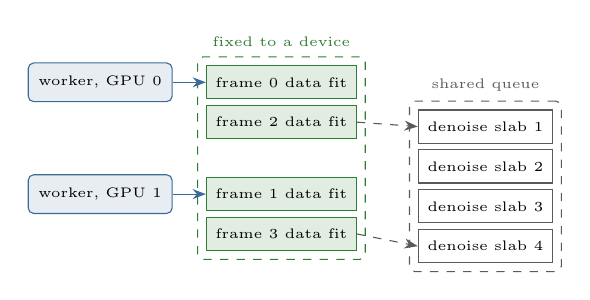
\begin{tikzpicture}[>=Stealth, node distance=4pt and 12pt,
          dev/.style={draw, rounded corners=2pt, fill=planAccent!12, draw=planAccent, minimum width=52pt, minimum height=14pt, font=\tiny},
          fixed/.style={draw, fill=safeGreen!14, draw=safeGreen, minimum width=48pt, minimum height=12pt, font=\tiny},
          any/.style={draw, fill=white, draw=inkGray, minimum width=48pt, minimum height=12pt, font=\tiny}]
        \node[dev] (g0) {worker, GPU 0};
        \node[dev, below=26pt of g0] (g1) {worker, GPU 1};
        \node[fixed, right=of g0] (f0) {frame 0 data fit};
        \node[fixed, below=2pt of f0] (f2) {frame 2 data fit};
        \node[fixed, right=of g1] (f1) {frame 1 data fit};
        \node[fixed, below=2pt of f1] (f3) {frame 3 data fit};
        \node[any, right=22pt of f0.east, yshift=-16pt] (q0) {denoise slab 1};
        \node[any, below=2pt of q0] (q1) {denoise slab 2};
        \node[any, below=2pt of q1] (q2) {denoise slab 3};
        \node[any, below=2pt of q2] (q3) {denoise slab 4};
        \node[draw=inkGray, dashed, rounded corners=2pt, fit=(q0)(q3), inner sep=3pt, label={[font=\tiny, inkGray]above:shared queue}] {};
        \node[draw=safeGreen, dashed, rounded corners=2pt, fit=(f0)(f3), inner sep=3pt, label={[font=\tiny, safeGreen]above:fixed to a device}] {};
        \draw[->, planAccent] (g0.east) -- (f0.west);
        \draw[->, planAccent] (g1.east) -- (f1.west);
        \draw[->, inkGray, dashed] (f2.east) -- (q0.west);
        \draw[->, inkGray, dashed] (f3.east) -- (q3.west);
      \end{tikzpicture}\\[6pt]
      \figcaption{One step on two GPUs, as the 4D model uses them.  Each
      frame's data fit is fixed to a device.  The denoising slabs accept
      any device and wait in the shared queue.  The \texttt{tasks} trace in
      \texttt{info} records the start and end time of every task and the
      worker that ran it.}
    \end{column}
  \end{columns}
  \source{\texttt{MACE.\_run\_threaded} and \texttt{resolve\_device\_pool} in \texttt{mbirtorch/mace.py}}
\end{frame}

% ---------------------------------------------------------------- what an agent is
\begin{frame}{What an agent is \hfill \macechip}
  \begin{columns}[T]
    \begin{column}{0.50\textwidth}
      {\footnotesize
      \head{The one requirement.}  An agent is a callable
      \texttt{agent(w, iteration)} that returns a tensor of the shape of
      \texttt{w} on the device of \texttt{w}.  The loop wraps it as one
      task over the whole array, fixed to the agent's \texttt{device}
      attribute when it has one.\par\vspace{5pt}
      \head{Splitting the work.}  An agent may instead provide
      \texttt{tasks(w, iteration)}, which returns a list of \texttt{Task}
      objects.  Each task computes one region of the output, and the
      tasks may run on different workers at the same
      time.\par\vspace{4pt}
      \sig{class}{mbirtorch.mace.Task}{run, device=None, region=None}
      \begin{params}
        \param{run}{callable}{\texttt{run(device)} computes the output over the region on that device}
        \param{device}{torch.device, optional}{the device the task must run on; None means any}
        \param{region}{tuple of slice, optional}{the slices the output covers; None means the whole array}
      \end{params}}
    \end{column}
    \begin{column}{0.48\textwidth}
      {\footnotesize
      \head{When a region cannot be added alone.}  Some agents produce
      output that depends on every region, for example a filter along an
      axis that the tasks split.  Such an agent sets
      \texttt{fold\_after\_all = True} and provides \texttt{pieces()}.
      Its tasks then return nothing and only compute.  After the last task
      of the step has run, the loop calls \texttt{pieces()}, which yields
      \texttt{(region, output)} pairs, and adds those.  The 4D data fit
      agent works this way: each frame is reconstructed on its own GPU,
      and the frame axis filter is applied across all frames
      afterward.\par\vspace{5pt}
      \head{Saving state.}  An agent may provide \texttt{state\_dict()}
      and \texttt{load\_state\_dict()}.  The loop then saves the agent's
      state with its own and restores it with its own.\par}
    \end{column}
  \end{columns}
  \source{docstrings of \texttt{MACE} and \texttt{Task} in \texttt{mbirtorch/mace.py}}
\end{frame}

% ---------------------------------------------------------------- example, tasks
\begin{frame}[fragile]{Example: an agent that splits its work into tasks \hfill \macechip}
  \begin{columns}[T]
    \begin{column}{0.56\textwidth}
\begin{lstlisting}
from mbirtorch import MACE, Task

class SlabDenoiser:
    def __init__(self, denoise, slab=32):
        self.denoise = denoise  # tensor -> tensor
        self.slab = slab

    def tasks(self, w, iteration=0):
        tasks = []
        for start in range(0, w.shape[0], self.slab):
            region = (slice(start, start + self.slab),)
            def run(device, region=region):
                out = self.denoise(w[region].to(device))
                return out.to(w.device)
            tasks.append(Task(run, region=region))
        return tasks

agents = [data_fit, SlabDenoiser(my_denoise)]
pool = ['cuda:0', 'cuda:1']
with MACE(agents, x0, devices=pool) as loop:
    x_bar, info = loop.run(max_iterations=30)
\end{lstlisting}
    \end{column}
    \begin{column}{0.42\textwidth}
      {\footnotesize
      \head{What happens in one step.}  For a volume of 512 slices the
      agent returns 16 tasks, one per slab of 32 slices.  None names a
      device, so all 16 go into the shared queue, and the two workers
      take them as they become free.  Each task copies its slab to its
      worker's GPU, denoises it, and returns the result on the device of
      \texttt{w}.  The loop adds each slab into the consensus as it
      arrives.\par\vspace{5pt}
      \head{Why this scales.}  No task holds the whole volume on a GPU.
      The slab size sets the memory one task needs, and the pool size
      sets how many run at once.\par\vspace{5pt}
      \head{No \texttt{\_\_call\_\_} is needed} once \texttt{tasks} is
      provided, because the loop runs the tasks and never calls the agent
      directly.\par}
    \end{column}
  \end{columns}
  \source{\texttt{Task}, \texttt{MACE.step} in \texttt{mbirtorch/mace.py}; \texttt{HyperplaneAgent.tasks} follows the same pattern}
\end{frame}

% ---------------------------------------------------------------- the agents, 1
\begin{frame}{The agents the package provides: data fit and denoiser \hfill \macechip}
  \vspace{2pt}
  \sig{class}{mbirtorch.mace.ForwardProxAgent}{model, sinogram, weights=None, sigma\_prox=None, inner\_iterations=3, init\_recon=None, device=None, partition\_advance=1.0, use\_warm\_start=True}
  \sigtext{The proximal map of the data fit term of one scan, through the
  model's \texttt{prox\_map}.  Each call runs \texttt{inner\_iterations}
  iterations of the reconstruction solver.  Over the loop the solver's
  partitions go from coarse to fine, \texttt{partition\_advance} entries
  per loop iteration.}
  \begin{params}
    \param{model, sinogram, weights}{}{the projection model on one device, the measured sinogram, and optional weights}
    \param{sigma\_prox}{float, optional}{the proximal strength; None uses the model's automatic value}
    \param{device}{optional}{a device to pin the model to; the sinogram and weights are placed on it once}
    \param{use\_warm\_start}{bool, optional}{start each call from the agent's previous output, or from its input when False}
  \end{params}
  \vspace{2pt}
  \sig{class}{mbirtorch.mace.QGGMRFDenoiserAgent}{image\_shape, sigma\_noise, pinned\_params=None, inner\_iterations=8, like\_model=None, use\_ror\_mask=False, device=None, use\_warm\_start=True}
  \sigtext{The qGGMRF prior on one volume, through \texttt{QGGMRFDenoiser}.
  The prior parameters are fixed at construction, so the agent is the same
  operator on every call and \texttt{sigma\_noise} is its one strength.}
  \begin{params}
    \param{pinned\_params}{dict, optional}{prior parameters to fix, such as \texttt{\{'sigma\_x': value\}}}
    \param{like\_model}{TomographyModel, optional}{a model whose device the denoiser copies; \texttt{device} takes precedence}
  \end{params}
  \source{class docstrings in \texttt{mbirtorch/mace.py}}
\end{frame}

% ---------------------------------------------------------------- the agents, 2
\begin{frame}{The agents the package provides: a prior on a 4D array \hfill \macechip}
  \vspace{2pt}
  \sig{class}{mbirtorch.mace.HyperplaneAgent}{axis, make\_stack\_denoiser, batch\_size=None, filter\_matrix=None, use\_warm\_start=False}
  \sigtext{The array has shape (frames, x, y, z).  Fixing one spatial
  axis at one index gives a 3D volume that holds every frame, called a
  hyperplane volume here.  The agent denoises the stack of all such volumes,
  so the prior couples neighboring frames as well as neighboring voxels.
  The work is split into tasks of \texttt{batch\_size} volumes, and any
  device of the pool may take a task.}
  \begin{params}
    \param{axis}{int}{the spatial axis that is fixed: 1, 2, or 3 in the (frames, x, y, z) order}
    \param{make\_stack\_denoiser}{callable}{\texttt{make\_stack\_denoiser(device)} returns the denoiser of a stack for that device, a callable \texttt{denoise(stack)} on a tensor of shape (volumes, frames, d1, d2).  One is made per worker and kept.}
    \param{batch\_size}{int, optional}{volumes per task.  None puts the whole orientation in one task.  The 4D model passes the number of volumes that fit its slab budget.}
    \param{filter\_matrix}{torch.Tensor, optional}{a square matrix of the size of the frame axis, applied along that axis before denoising, such as the one from \texttt{temporal\_filter\_matrix}}
    \param{use\_warm\_start}{bool, optional}{keep the previous output, one array of the input's size, and pass the matching slab to the denoiser as its start}
  \end{params}
  \vfill
  \footnoteline{Each of the three agents needs a model on one device.  A
  model on several devices returns its output divided across them, which
  the loop cannot add into one array, so the agent refuses it with a named
  error.}
  \source{class docstring of \texttt{HyperplaneAgent} in \texttt{mbirtorch/mace.py}}
\end{frame}

% ---------------------------------------------------------------- example, one call
\begin{frame}[fragile]{Example: a data fit and a denoiser agree on one volume \hfill \macechip}
  \begin{columns}[T]
    \begin{column}{0.56\textwidth}
\begin{lstlisting}
import mbirtorch
from mbirtorch import ForwardProxAgent, QGGMRFDenoiserAgent
from mbirtorch.mace import mace

# The usual 3D model, on one GPU.
model = mbirtorch.ConeBeamModel(
    sino.shape, angles, source_detector_dist=sdd,
    source_iso_dist=sid)
model.configure_devices(devices=['cuda:0'])
x0, _ = model.recon(sino)

# Two agents with equal weight.
agents = [
    ForwardProxAgent(model, sino, weights=w),
    QGGMRFDenoiserAgent(x0.shape, sigma_noise=0.02,
                        like_model=model)]
x, info = mace(agents, x0, mu=[0.5, 0.5],
               num_iterations=30)
\end{lstlisting}
    \end{column}
    \begin{column}{0.42\textwidth}
      {\footnotesize
      \head{The one call form.}  \texttt{mace} constructs the loop, runs a
      fixed number of steps on the calling thread, and returns the average
      and the traces.\par\vspace{5pt}
      \head{The two agents.}  The first holds the model, the sinogram, and
      the weights.  The second holds a denoiser of the volume's shape on
      the same device as the model.  Its strength is the noise level
      \texttt{sigma\_noise}.\par\vspace{5pt}
      \head{The result} \texttt{x} is the consensus average.  The dict
      \texttt{info} holds one entry per step: the percent change and the
      spread of the agents.\par\vspace{5pt}
      \head{A user's own agent} is any \texttt{f(w, iteration)} that
      returns a tensor of the shape of \texttt{w}.  It goes into the same
      list.\par}
    \end{column}
  \end{columns}
  \source{\texttt{mace} and the agent docstrings in \texttt{mbirtorch/mace.py}}
\end{frame}

% ---------------------------------------------------------------- example, class form
\begin{frame}[fragile]{Example: the class form, with a device pool and a checkpoint \hfill \macechip}
  \begin{columns}[T]
    \begin{column}{0.56\textwidth}
\begin{lstlisting}
import torch
from mbirtorch import MACE

with MACE(agents, x0, mu=[0.5, 0.5], rho=0.5,
          devices=['cuda:0', 'cuda:1']) as loop:
    loop.run(max_iterations=10)
    torch.save(loop.state_dict(), 'state.pt')

# Later, a new loop with the same agents and shape.
with MACE(agents, x0, mu=[0.5, 0.5], rho=0.5,
          devices=['cuda:0', 'cuda:1']) as loop:
    loop.load_state_dict(torch.load('state.pt'))
    x_bar, info = loop.run(max_iterations=30)
    x = x_bar.clone()  # the buffer belongs to the loop
\end{lstlisting}
    \end{column}
    \begin{column}{0.42\textwidth}
      {\footnotesize
      \head{The device pool.}  Two GPUs are named, so the loop runs two
      worker threads.  Agents that split their work into tasks spread
      them over both.\par\vspace{5pt}
      \head{The checkpoint.}  \texttt{state\_dict} returns the agent
      inputs, the average, the iteration count, the traces, and each
      agent's own state.  \texttt{torch.save} writes it to
      disk.\par\vspace{5pt}
      \head{The resume.}  The second loop continues from step 10 to step
      30.  It keeps its own \texttt{mu} and \texttt{rho} and warns when
      the saved ones differ.\par\vspace{5pt}
      \head{The context manager} stops the worker threads on exit.  A
      loop used without it is closed with \texttt{close()}.\par}
    \end{column}
  \end{columns}
  \source{\texttt{MACE.run}, \texttt{MACE.state\_dict}, \texttt{MACE.load\_state\_dict} in \texttt{mbirtorch/mace.py}}
\end{frame}

% ================================================================ PART 2
\section{Part 2: 4D reconstruction with \texttt{MACE4DModel}}

% ---------------------------------------------------------------- the problem
\begin{frame}{The problem and the idea \hfill \fourdchip}
  \begin{columns}[T]
    \begin{column}{0.50\textwidth}
      {\footnotesize
      \head{The problem.}  When the object moves during one continuous
      scan, one volume cannot represent it.  A volume from a short window
      of views alone is poor.\par\vspace{5pt}
      \head{The idea.}  The views are divided into overlapping windows,
      one per time frame, and one volume is reconstructed per frame.  The
      frames are reconstructed together, so each frame is informed by its
      neighbors in time.\par\vspace{5pt}
      \head{The four agents.}  The first is the data fit of every frame.
      The other three are qGGMRF denoisers on the volumes (t, x, y),
      (t, y, z), and (t, x, z), which hold the frame axis and two spatial
      axes, so they smooth along time as well as along
      space.\par\vspace{5pt}
      \head{The frame axis filter.}  Overlapping windows produce a periodic
      variation along the frame axis.  A filter with that period removes
      it from the data fit outputs.\par}
    \end{column}
    \begin{column}{0.48\textwidth}
      \centering
      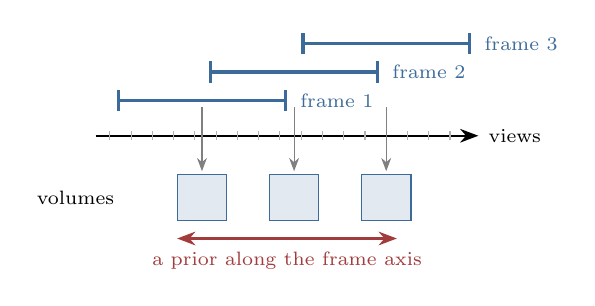
\begin{tikzpicture}[>=Stealth, scale=0.9]
        \draw[->, thick] (0,0) -- (5.4,0) node[right, font=\scriptsize] {views};
        \foreach \x in {0.2,0.5,...,5.1} { \draw[gray!60] (\x,-0.06) -- (\x,0.06); }
        \foreach \i/\y in {0/0.5, 1/0.9, 2/1.3} {
          \pgfmathsetmacro{\xa}{0.3+1.3*\i}
          \pgfmathsetmacro{\xb}{\xa+2.4}
          \draw[planAccent, very thick, |-|] (\xa,\y) -- (\xb,\y);
          \node[planAccent, font=\scriptsize, anchor=west] at (\xb+0.05,\y) {frame \the\numexpr\i+1\relax};
        }
        \foreach \i in {0,1,2} {
          \pgfmathsetmacro{\xc}{0.3+1.3*\i+1.2}
          \draw[->, gray] (\xc,0.4) -- (\xc,-0.5);
          \draw[fill=planAccent!15, draw=planAccent] (\xc-0.35,-1.2) rectangle (\xc+0.35,-0.55);
        }
        \node[font=\scriptsize, anchor=east] at (0.4,-0.87) {volumes};
        \draw[<->, axialBrick, thick] (1.15,-1.45) -- (4.25,-1.45);
        \node[axialBrick, font=\scriptsize, anchor=north] at (2.7,-1.5) {a prior along the frame axis};
      \end{tikzpicture}\\[4pt]
      \figcaption{Overlapping windows of views, one per time frame.  With
      six frames per rotation and an overlap factor of two, each frame
      spans 120 degrees and each view belongs to two frames.}
    \end{column}
  \end{columns}
  \source{module and class docstrings of \texttt{mbirtorch/mace4d.py}}
\end{frame}

% ---------------------------------------------------------------- the class, part 1
\begin{frame}{The \texttt{MACE4DModel} class: constructing it \hfill \fourdchip}
  \vspace{0pt}
  {\small The constructor takes the model of the whole scan and divides its
  views into frames.  Nothing is reconstructed until \texttt{recon} is
  called.}\par\vspace{2pt}
  \sig{class}{mbirtorch.mace4d.MACE4DModel}{ct\_model, frames\_per\_rotation=6, frame\_overlap\_factor=2.0, num\_frames=None}
  \begin{params}
    \param{ct\_model}{TomographyModel}{the model of the full scan, a \texttt{ConeBeamModel} or a \texttt{ParallelBeamModel} with one angle per view, in time order.  Its geometry and regularization parameters are set before construction.}
    \param{frames\_per\_rotation}{int, optional}{frames per full rotation.  This is also the period of the frame axis filter.}
    \param{frame\_overlap\_factor}{float, optional}{the number of frames that cover any one view.  Each frame spans \texttt{frame\_overlap\_factor * 360 / frames\_per\_rotation} degrees.}
    \param{num\_frames}{int, optional}{reconstruct only this many frames, counted from the start of the scan.  None means every frame.}
  \end{params}
  \vspace{3pt}
  {\scriptsize
  \begin{tabular}{@{}>{\raggedright\arraybackslash}p{0.30\linewidth}@{\hspace{6pt}}>{\raggedright\arraybackslash}p{0.66\linewidth}@{}}
    \speclabel{attributes} & \\[2pt]
    \texttt{model\_list}, \texttt{view\_slices} & one model per frame, and the views of each frame \\[2pt]
    \texttt{num\_frames} & the number of frames \\[2pt]
    \texttt{recon\_shape}, \texttt{sinogram\_shape} & the shape of one frame's volume, and the shape of the full sinogram \\
  \end{tabular}}
  \vfill
  \footnoteline{The class follows the pattern of the other mbirtorch models:
  numpy in, numpy out, and GPU use is the library's responsibility.}
  \source{class docstring of \texttt{MACE4DModel} in \texttt{mbirtorch/mace4d.py}}
\end{frame}

% ---------------------------------------------------------------- the class, part 2
\begin{frame}{The \texttt{MACE4DModel} class: its methods \hfill \fourdchip}
  \vspace{0pt}
  {\scriptsize
  \begin{tabular}{@{}>{\raggedright\arraybackslash}p{0.30\linewidth}@{\hspace{6pt}}>{\raggedright\arraybackslash}p{0.66\linewidth}@{}}
    \texttt{set\_params(**kwargs)} & the reconstruction parameters by keyword; a later slide lists them \\[2pt]
    \texttt{get\_params(name)} & read one back \\[2pt]
    \texttt{set\_device\_pool(devices=None)} & the devices \texttt{recon} spreads its work over, in any form the MACE pool accepts.  Each frame's data fit is fixed to one device in turn, and any device takes a denoising task. \\
  \end{tabular}}
  \vspace{4pt}
  \sig{method}{recon}{sinogram, weights=None, init\_recon=None, max\_iterations=10, stop\_threshold\_change\_pct=0.2, init\_dir=None, log\_dir=None}
  \sigtext{Reconstruct one volume per time frame from the sinogram of the scan.}
  \begin{params}
    \param{sinogram}{numpy or tensor}{the full sinogram, of shape (views, rows, channels)}
    \param{weights}{numpy or tensor, optional}{positive weights of the sinogram's shape.  None means unit weights.}
    \param{init\_recon}{numpy, optional}{the initial 4D image of shape (frames, x, y, z).  None reads it from \texttt{init\_dir} when one is there, and otherwise reconstructs each frame alone.}
    \param{max\_iterations, stop\_threshold\_change\_pct}{}{consensus iterations, and the percent change of the 4D image in one iteration below which the loop stops}
    \param{init\_dir, log\_dir}{str, optional}{a directory for the cached initial image, and a directory for the log files}
  \end{params}
  \returns{\texttt{(recon\_4d, recon\_dict)}, a numpy array of shape (frames, x, y, z) and a dict with the run settings and the timing.}
  \source{\texttt{MACE4DModel.recon} in \texttt{mbirtorch/mace4d.py}}
\end{frame}

% ---------------------------------------------------------------- inside recon
\begin{frame}{What \texttt{m4d.recon} does inside \hfill \fourdchip}
  \begin{columns}[T]
    \begin{column}{0.54\textwidth}
      {\footnotesize
      The method runs seven steps.
      \begin{enumerate}\setlength{\itemsep}{1pt}
        \item Check the shapes of the sinogram, the weights, and the
          initial image.
        \item Build the frame axis filter, or turn it off with a warning
          when the frames are fewer than the period.
        \item Make one \texttt{ForwardProxAgent} per frame, on its device
          of the pool.
        \item Get the initial 4D image: the one given, the cached one, or
          each frame reconstructed alone.
        \item Set the denoiser strengths from the initial image, unless
          they were given.
        \item Make the three \texttt{HyperplaneAgent}s, divided into slabs
          of a fixed size.
        \item Run the \texttt{MACE} loop on the pool and write the logs
          after each step.
      \end{enumerate}}
    \end{column}
    \begin{column}{0.44\textwidth}
      \centering
      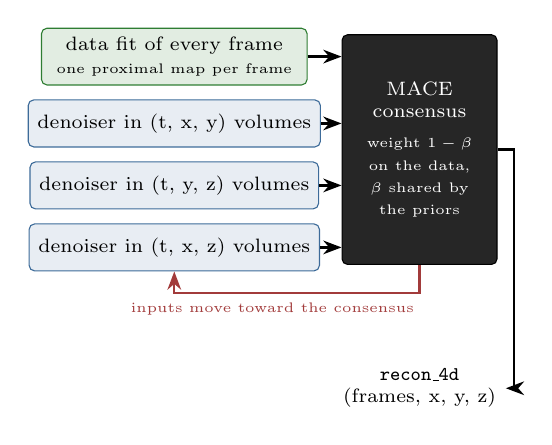
\begin{tikzpicture}[>=Stealth, node distance=5pt and 10pt,
          agent/.style={draw, rounded corners=2pt, minimum width=96pt, minimum height=17pt, font=\scriptsize, align=center},
          data/.style={agent, fill=safeGreen!14, draw=safeGreen},
          prior/.style={agent, fill=planAccent!12, draw=planAccent},
          cons/.style={draw, rounded corners=2pt, fill=barGray, text=white, minimum width=56pt, font=\scriptsize, align=center, inner ysep=0pt}]
        \node[data] (d) {data fit of every frame\\ \tiny one proximal map per frame};
        \node[prior, below=of d] (p1) {denoiser in (t, x, y) volumes};
        \node[prior, below=of p1] (p2) {denoiser in (t, y, z) volumes};
        \node[prior, below=of p2] (p3) {denoiser in (t, x, z) volumes};
        \path (d.north east) -- (p3.south east) coordinate[midway] (mid);
        \node[cons, anchor=west, minimum height=83pt] (c) at ($(mid)+(10pt,0)$) {MACE\\ consensus\\[3pt] \tiny weight $1-\beta$\\ \tiny on the data,\\ \tiny $\beta$ shared by\\ \tiny the priors};
        \foreach \a in {d,p1,p2,p3} { \draw[->, thick] (\a.east) -- (c.west |- \a.east); }
        \draw[->, axialBrick, thick] (c.south) -- ++(0,-10pt) -| (p3.south)
          node[pos=0.3, below, font=\tiny, axialBrick] {inputs move toward the consensus};
        \node[below=34pt of c, font=\scriptsize, align=center] (out) {\texttt{recon\_4d}\\ (frames, x, y, z)};
        \draw[->, thick] (c.east) -- ++(6pt,0) |- (out.east);
      \end{tikzpicture}\\[4pt]
      \figcaption{The four agents of the 4D loop.  The three denoisers
      share the prior weight equally unless three weights are given.}
    \end{column}
  \end{columns}
  \source{\texttt{MACE4DModel.recon} in \texttt{mbirtorch/mace4d.py}}
\end{frame}

% ---------------------------------------------------------------- parameters
\begin{frame}{The parameters of \texttt{m4d.set\_params} \hfill \fourdchip}
  \vspace{0pt}
  {\scriptsize
  \begin{tabular}{@{}>{\raggedright\arraybackslash}p{0.11\linewidth}@{\hspace{5pt}}>{\raggedright\arraybackslash}p{0.27\linewidth}@{\hspace{5pt}}>{\raggedright\arraybackslash}p{0.58\linewidth}@{}}
    \speclabel{group} & \speclabel{parameter and default} & \speclabel{meaning} \\[2pt]
    consensus & \texttt{mace\_prior\_weight=0.5} & the total weight of the three priors, or one weight each; the data fit gets the rest \\
      & \texttt{rho\_mann=0.5} & the step of the consensus iteration \\[2pt]
    \rowrule
    data fit & \texttt{prox\_num\_iterations=3} & solver iterations of each data fit call \\
      & \texttt{sigma\_prox=None} & the strength of every data fit call; None sets it from the data \\
      & \texttt{prox\_warm\_start=True} & each call starts from the frame's previous output \\
      & \texttt{prox\_partition\_advance=1.0} & how fast the solver's partitions go from coarse to fine \\
      & \texttt{prox\_stop\_threshold=0.02} & the stop threshold, in percent, of the per frame initialization \\[2pt]
    \rowrule
    denoisers & \texttt{sigma\_noise=None} & the noise level of all three; None estimates it from the initial image \\
      & \texttt{sigma\_x}, \texttt{sharpness=0.0} & the prior strength of all three, and a scale on its automatic estimate \\
      & \texttt{nbr\_weight\_time=1.0} & the weight of a frame neighbor against a spatial neighbor; it replaces \texttt{qggmrf\_nbr\_wts}, which is refused here \\
      & \texttt{denoiser\_warm\_start=False} & each sweep starts from its previous output; costs one full size array per orientation \\[2pt]
    \rowrule
    filter & \texttt{dejitter=True}, \texttt{dejitter\_verbose=0} & apply the frame axis filter, and log the periods it removes \\[2pt]
    \rowrule
    memory, output & \texttt{denoise\_slab\_gb=2.0} & the size of the stack of volumes one denoiser task sweeps; a task holds about three such arrays \\
      & \texttt{verbose=1} & 0 is silent, 1 reports progress \\
  \end{tabular}}
  \source{\texttt{MACE4DModel.set\_params} in \texttt{mbirtorch/mace4d.py}}
\end{frame}

% ---------------------------------------------------------------- example
\begin{frame}[fragile]{Example: a 4D reconstruction on two GPUs \hfill \fourdchip}
  \begin{columns}[T]
    \begin{column}{0.56\textwidth}
\begin{lstlisting}
import mbirtorch
from mbirtorch import MACE4DModel

# The model of the full scan, one angle per view.
ct_model = mbirtorch.ConeBeamModel(
    sino.shape, angles, source_detector_dist=sdd,
    source_iso_dist=sid)
ct_model.set_params(sharpness=1.0)

# Six frames per rotation, each view in two frames.
m4d = MACE4DModel(ct_model, frames_per_rotation=6,
                  frame_overlap_factor=2.0)
m4d.set_params(mace_prior_weight=0.5, rho_mann=0.5)
m4d.set_device_pool(2)

w = mbirtorch.gen_weights(sino, 'transmission_root')
recon_4d, recon_dict = m4d.recon(
    sino, weights=w, max_iterations=10,
    init_dir='./init', log_dir='./logs')

print(recon_4d.shape)  # (num_frames, x, y, z)
frame_3 = recon_4d[3]  # one volume
\end{lstlisting}
    \end{column}
    \begin{column}{0.42\textwidth}
      {\footnotesize
      \head{What the script does.}  The first block builds the usual 3D
      model of the scan.  The second wraps it as a 4D model, sets the two
      consensus parameters, and names two GPUs.  The third runs the
      reconstruction.\par\vspace{5pt}
      \head{The two directories are optional.}  \texttt{init\_dir} caches
      the per frame initialization, so a second run with other parameters
      skips it.  \texttt{log\_dir} receives three files, described on the
      next slide.\par\vspace{5pt}
      \head{The pool line is optional too.}  If
      \texttt{m4d.set\_device\_pool(2)} is left out, \texttt{recon} uses
      every GPU, or the CPU when there is none.  The rest of the script is
      the same either way.\par}
    \end{column}
  \end{columns}
  \source{docstring examples of \texttt{MACE4DModel} in \texttt{mbirtorch/mace4d.py}}
\end{frame}

% ---------------------------------------------------------------- outputs
\begin{frame}{What \texttt{m4d.recon} returns and writes \hfill \fourdchip}
  \begin{columns}[T]
    \begin{column}{0.50\textwidth}
      {\footnotesize
      \head{The return value} is \texttt{(recon\_4d, recon\_dict)}.\par\vspace{3pt}
      {\scriptsize
      \begin{tabular}{@{}>{\raggedright\arraybackslash}p{0.28\linewidth}@{\hspace{5pt}}>{\raggedright\arraybackslash}p{0.66\linewidth}@{}}
        \texttt{recon\_4d} & numpy float32 of shape (frames, x, y, z) \\[2pt]
        \texttt{'recon\_params'} & the run settings: the pool, where the initial image came from, the denoiser strengths and their source, the filter, the iterations completed \\[2pt]
        \texttt{'timing'} & one row per iteration, the same rows as the timing log \\[2pt]
        \texttt{'notes'} & the completion time \\[2pt]
        \texttt{'model\_params'} & a copy of the model's parameters \\
      \end{tabular}}\par\vspace{7pt}
      \head{The initialization cache.}  With \texttt{init\_dir}, the per
      frame initial image is read from \texttt{init\_recon.npy} when it is
      there and written otherwise.\par}
    \end{column}
    \begin{column}{0.48\textwidth}
      {\footnotesize
      \head{The log files} are written to \texttt{log\_dir} after every
      iteration, so a run that stops early still has them.\par\vspace{3pt}
      {\scriptsize
      \begin{tabular}{@{}>{\raggedright\arraybackslash}p{0.26\linewidth}@{\hspace{5pt}}>{\raggedright\arraybackslash}p{0.68\linewidth}@{}}
        \texttt{run\_info.txt} & the run settings as text, one per line \\[2pt]
        \texttt{timing\_log.csv} & per iteration: the sum of the data fit task times, the sum of the denoising task times, the makespan, the wall time of the step, the percent change, and the mean number of denoiser iterations \\[2pt]
        \texttt{task\_log.csv} & per task: the iteration, the kind (\texttt{prox} or \texttt{denoise}), the frame or orientation, the slab, the worker, and the start and end times within the step \\
      \end{tabular}}\par\vspace{7pt}
      \head{The makespan} is the time from the start of the step to the
      end of its last task, that is the wall time of the parallel part of
      the step.  The two sums count work on all workers, so their total
      exceeds the makespan when the workers run in parallel.  The sums
      over the makespan times the number of workers is the GPU busy
      time.\par}
    \end{column}
  \end{columns}
  \source{\texttt{MACE4DModel.recon} in \texttt{mbirtorch/mace4d.py}}
\end{frame}

% ---------------------------------------------------------------- the filter functions
\begin{frame}[fragile]{Two helper functions: the frame axis filter \hfill \fourdchip}
  \begin{columns}[T]
    \begin{column}{0.52\textwidth}
      {\footnotesize
      \sig{function}{mbirtorch.temporal\_filter\_matrix}{num\_frames, period, harmonics=True, band\_width=1}
      Returns the filter as one square matrix of size \texttt{num\_frames}.
      Multiplying along the frame axis applies the filter.\par\vspace{4pt}
      \head{How the band works.}  The filter acts on the type I cosine
      transform of the frame axis, which has $N$ modes for $N$ frames, and
      mode $m$ has a period of $2(N-1)/m$ frames.  For each period to
      remove, the mode nearest that period is set to zero, together with
      \texttt{band\_width} modes on each side of it.  A band that would
      reach past the first or last mode is cut at that end.
      \texttt{harmonics=True} also removes every harmonic with a period of
      at least two frames.\par\vspace{4pt}
      \head{The ends of the frame axis.}  The type I cosine transform
      treats the frames as mirrored at both ends, so no frame wraps around
      to the other end and no zeros are added.\par}
    \end{column}
    \begin{column}{0.46\textwidth}
\begin{lstlisting}
import torch
from mbirtorch import temporal_filter_matrix
from mbirtorch import apply_temporal_filter

num_frames = recon_4d.shape[0]
F = temporal_filter_matrix(num_frames, period=6)
print(F.shape)  # (num_frames, num_frames)

x = torch.as_tensor(recon_4d)
x_filtered = apply_temporal_filter(x, F, axis=0)

# What the filter removed.
removed = x - x_filtered
\end{lstlisting}
      \vspace{4pt}
      {\footnotesize
      \sig{function}{mbirtorch.apply\_temporal\_filter}{x, matrix, axis=0}
      Applies the matrix along one axis of a tensor and returns a new
      tensor.\par\vspace{4pt}
      \head{Inside the model}, \texttt{recon} builds this matrix with the
      period \texttt{frames\_per\_rotation}.\par}
    \end{column}
  \end{columns}
  \source{docstrings of the two functions in \texttt{mbirtorch/mace4d.py}}
\end{frame}

% ================================================================ summary
\begin{frame}{Where the code is, and a summary}
  \vspace{0pt}
  {\footnotesize
  \head{The files.}  \texttt{mbirtorch/mace.py} holds the loop, the task
  class, the three agents, the pool helper, and the one call function.
  \texttt{mbirtorch/mace4d.py} holds the 4D model and the two filter
  functions.  The tests are \texttt{tests/test\_mace.py} and
  \texttt{tests/test\_mace4d.py}.  All of it is on branch
  \texttt{mace\_4d\_dev}.\par\vspace{5pt}
  \head{The names a user imports}, as \texttt{from mbirtorch import ...}:
  \begin{itemize}\setlength{\itemsep}{1pt}
    \item the loop and its pieces: \texttt{MACE}, \texttt{Task},
      \texttt{resolve\_device\_pool};
    \item the agents: \texttt{ForwardProxAgent},
      \texttt{QGGMRFDenoiserAgent}, \texttt{HyperplaneAgent};
    \item 4D reconstruction: \texttt{MACE4DModel},
      \texttt{temporal\_filter\_matrix}, \texttt{apply\_temporal\_filter};
    \item the one call loop is \texttt{from mbirtorch.mace import mace},
      since \texttt{mbirtorch.mace} names the module.
  \end{itemize}\vspace{3pt}
  \head{In two sentences.}  \texttt{MACE} runs several agents to
  agreement on one image, and any function from an image to an image is
  an agent.  \texttt{MACE4DModel} uses that loop with four agents to
  reconstruct one volume per time frame, with the usual mbirtorch
  pattern of numpy in and numpy out.\par\vspace{5pt}
  }
  \source{\texttt{mbirtorch/\_\_init\_\_.py}}
\end{frame}

% ================================================================ status
\begin{frame}{Status: timing on a real scan, and what remains}
  \vspace{0pt}
  {\small Phantom\_30s\_Run1, 99 frames, full resolution, four H100s, 2026-09-17.}\par\vspace{3pt}
  {\footnotesize
  \begin{tabular}{@{}>{\raggedright\arraybackslash}p{0.40\linewidth}@{\hspace{6pt}}r@{\hspace{14pt}}r@{\hspace{14pt}}>{\raggedright\arraybackslash}p{0.22\linewidth}@{}}
    \speclabel{per iteration, steady state} & \speclabel{mbirjax} & \speclabel{mbirtorch} & \\[3pt]
    iteration total & 387.2 s & 172.5 s & 2.24 times faster \\[1pt]
    makespan & 201.6 s & 170.2 s & 1.18 times faster \\[1pt]
    denoise, summed over workers & 421.8 s & 67.6 s & 6.2 times faster \\[1pt]
    data fit, summed over workers & 202.4 s & 609.2 s & 3.0 times slower \\[1pt]
    GPU busy time, while tasks run & 77.3\% & 99.3\% & \\[1pt]
    GPU busy time, whole iteration & 42.0\% & 97.8\% & \\[1pt]
    \rowrule
    \textbf{loop total, 10 iterations} & \textbf{68.0 min} & \textbf{25.8 min} & \textbf{2.64 times faster} \\
  \end{tabular}}\par\vspace{6pt}
  {\footnotesize
  \head{The two busy times} are the summed worker time divided by four
  times a span.  The first uses the makespan and asks: while tasks were
  running, did some GPUs finish early and wait for the others?  The
  second uses the whole iteration and also counts the stretch when no
  task runs at all, the consensus update and the bookkeeping.  mbirjax
  spreads its tasks fairly well but leaves the GPUs idle for 185.6 s of
  every iteration, about half of it.  In mbirtorch that stretch is
  2.3 s.\par\vspace{2pt}
  \head{Still to do.}  The documentation pages, and a demo in the
  package's demo folder.}
  \source{the 2026-09-17 cluster run, \texttt{timing\_log.csv} under \texttt{lilly\_exp/nsi/2026/0917/logs/}}
\end{frame}

\end{document}
